%%
%%
%%
%%

%% [intro]

The NIKA2 beam pattern mainly depends on the IRAM 30m telescope and NIKA2 internal optical system characteristics, whereas the detectors themselve might have an impact at sub-dominant level (through e.g. time constants or correlated noises). In this section, we characterize both the full beam pattern including error beams up to angular scales of 10 arcmin, and the main beam, which is modeled as an elliptical Gaussian.

%%[Full beam pattern]
\subsection{Full beam pattern}

\subsubsection{Deep beam maps}
We present the two-dimensional distribution of the beam in Fig.~\ref{fig:beam}. We primary use a map obtained from a combination of deep observations of strong point sources collected during \emph{NIKA2-run8} and \emph{run9}. Namely, we use 'beammap' OTF scans of Uranus (scan id '20170125s223' and '20170125s243'),  Neptune ('20170224s177') and the bright quasar 3C84 ('20170226s415'). However, we checked the stability of our results on single scan maps, combinations of scans for a single source, and combinations of shallower scans but spanning a large range of scanning direction. The data processing includes a mitigation of the correlated noise, which mainly originates from the atmosphere.  We primarly use a subtraction of a common mode estimated from the most correlated detectors (the so-called 'cm one block' method). However, other methods are tested for assessing the immunity of our results to noise residuals.

\begin{figure}
\begin{center}
  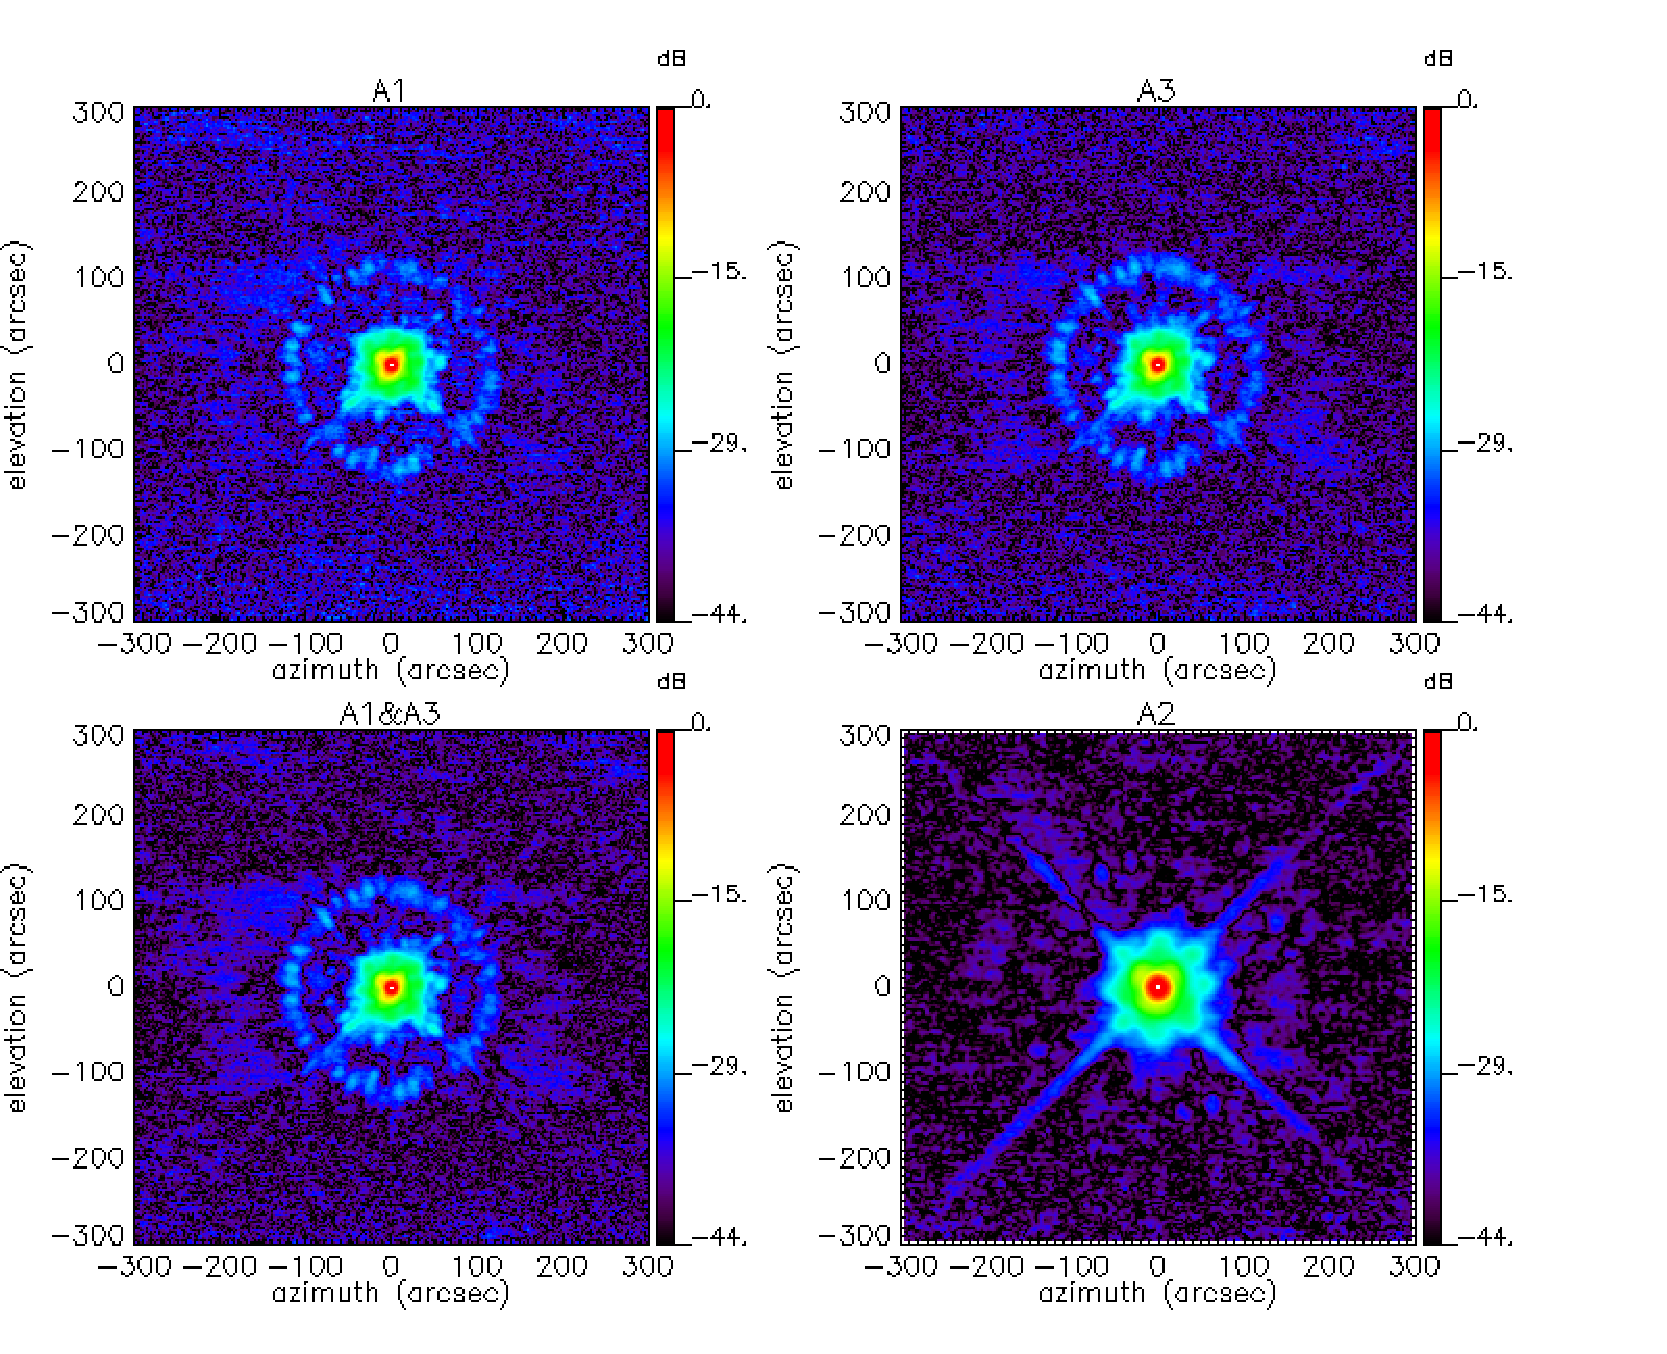
\includegraphics[clip, angle=0, scale=0.4]{Figures/Lobe_map_Combo_v2_dB.pdf}
 \caption{Beam pattern. From upper left to lower right, beam maps of array 1 (labeled 'A1'), array 3 ('A3'), the combination of the 1.15mm arrays ('A1$\&$3') and the 2mm array ('A2') are shown in decibel. These maps, which consist of normalized combination of four long OTF scans of bright point sources, are in celestial coordinates and cover a sky area which extend over 10 arcmin.}
\label{fig:beam}
\end{center}
\end{figure}


The deep NIKA2 beam maps reveal some noticeable features, which are shown in Fig.~\ref{fig:features}. 

\begin{figure}
\begin{center}
  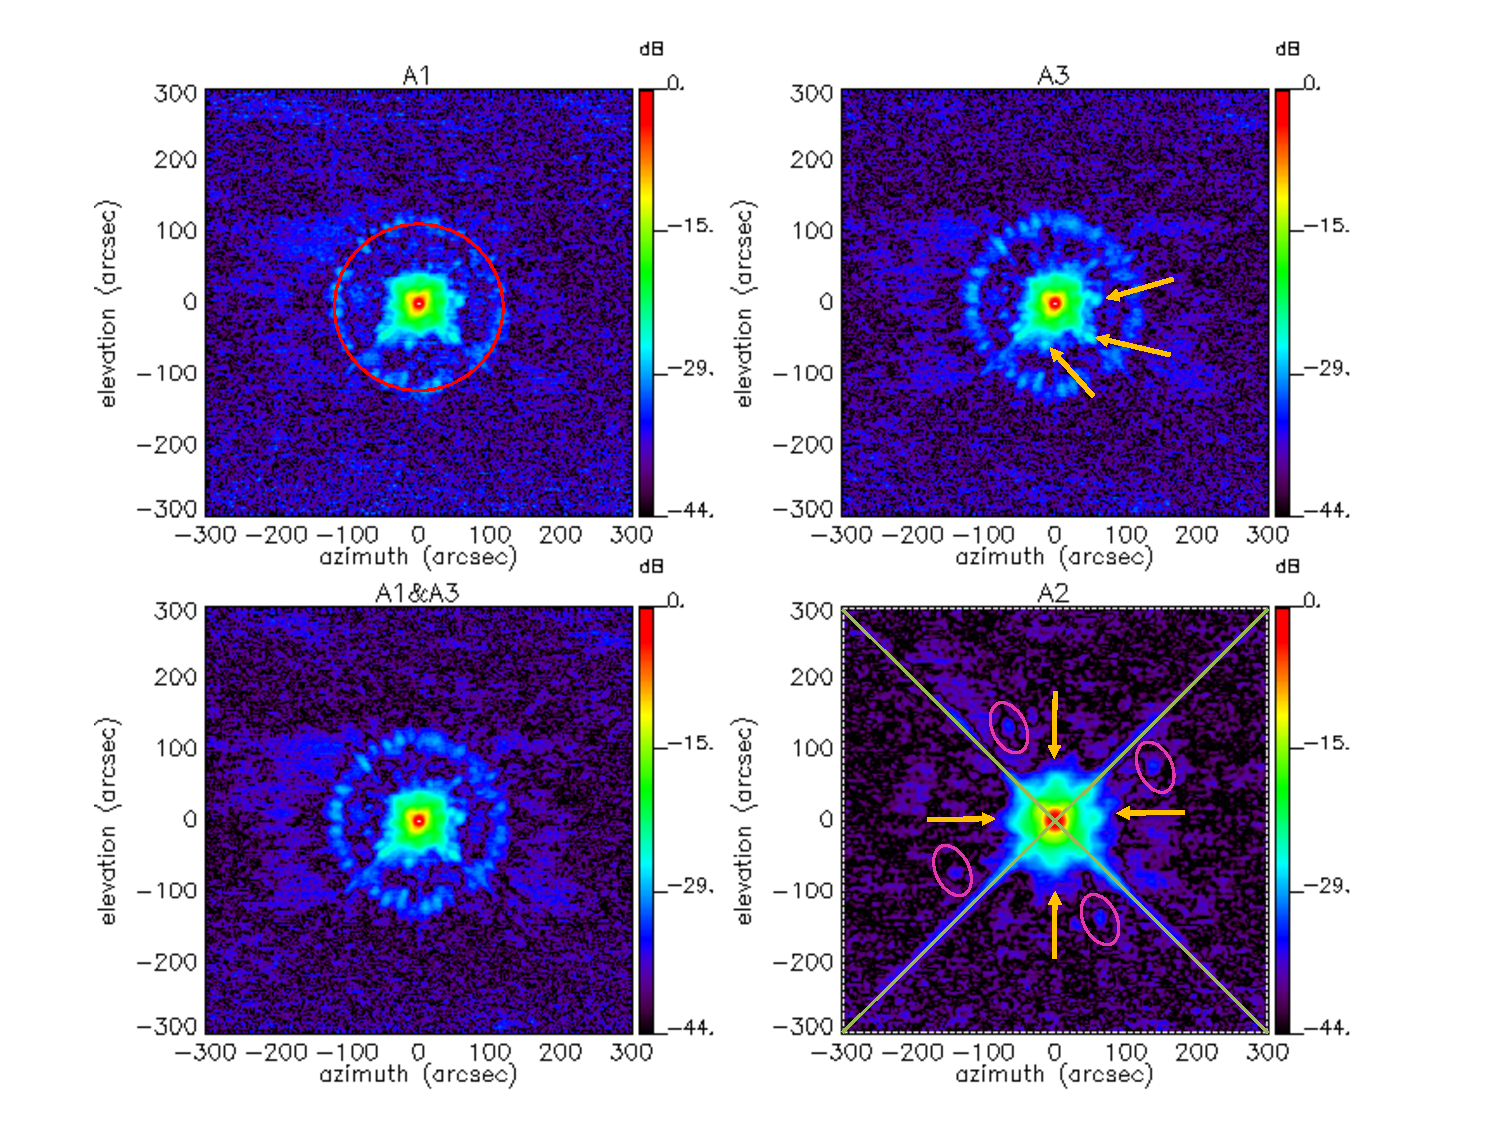
\includegraphics[clip, angle=0, scale=0.4]{Figures/Beams_features.pdf}
\caption{Noticeable features of NIKA2 beam pattern. Red circle: diffraction ring seen in 1-mm maps (the spokes are presumably caused by radial and azimuthal panel buckling (cf. Fig.4 in Greve et al. 2010)); Perpendicular green lines: diffraction pattern caused by quadrupod secondary support structure (prominently seen in 2mm maps); Yellow arrows in the upper right pannel: pattern of 3 spikes seen in 1mm maps of unknown origin; Yellow arrows in the lower right pannel: four symmetrical spokes of the first errorbeam; Pink ellipses: 4 spikes seen in 2mm maps.}
\label{fig:features}
\end{center}
\end{figure}

We further quantify the relative level of the main beam, the first error beam and other features seen in the 2D beam pattern using radial cuts.

[FIGURE JEAN-FRANCOIS]

\begin{figure}
\begin{center}
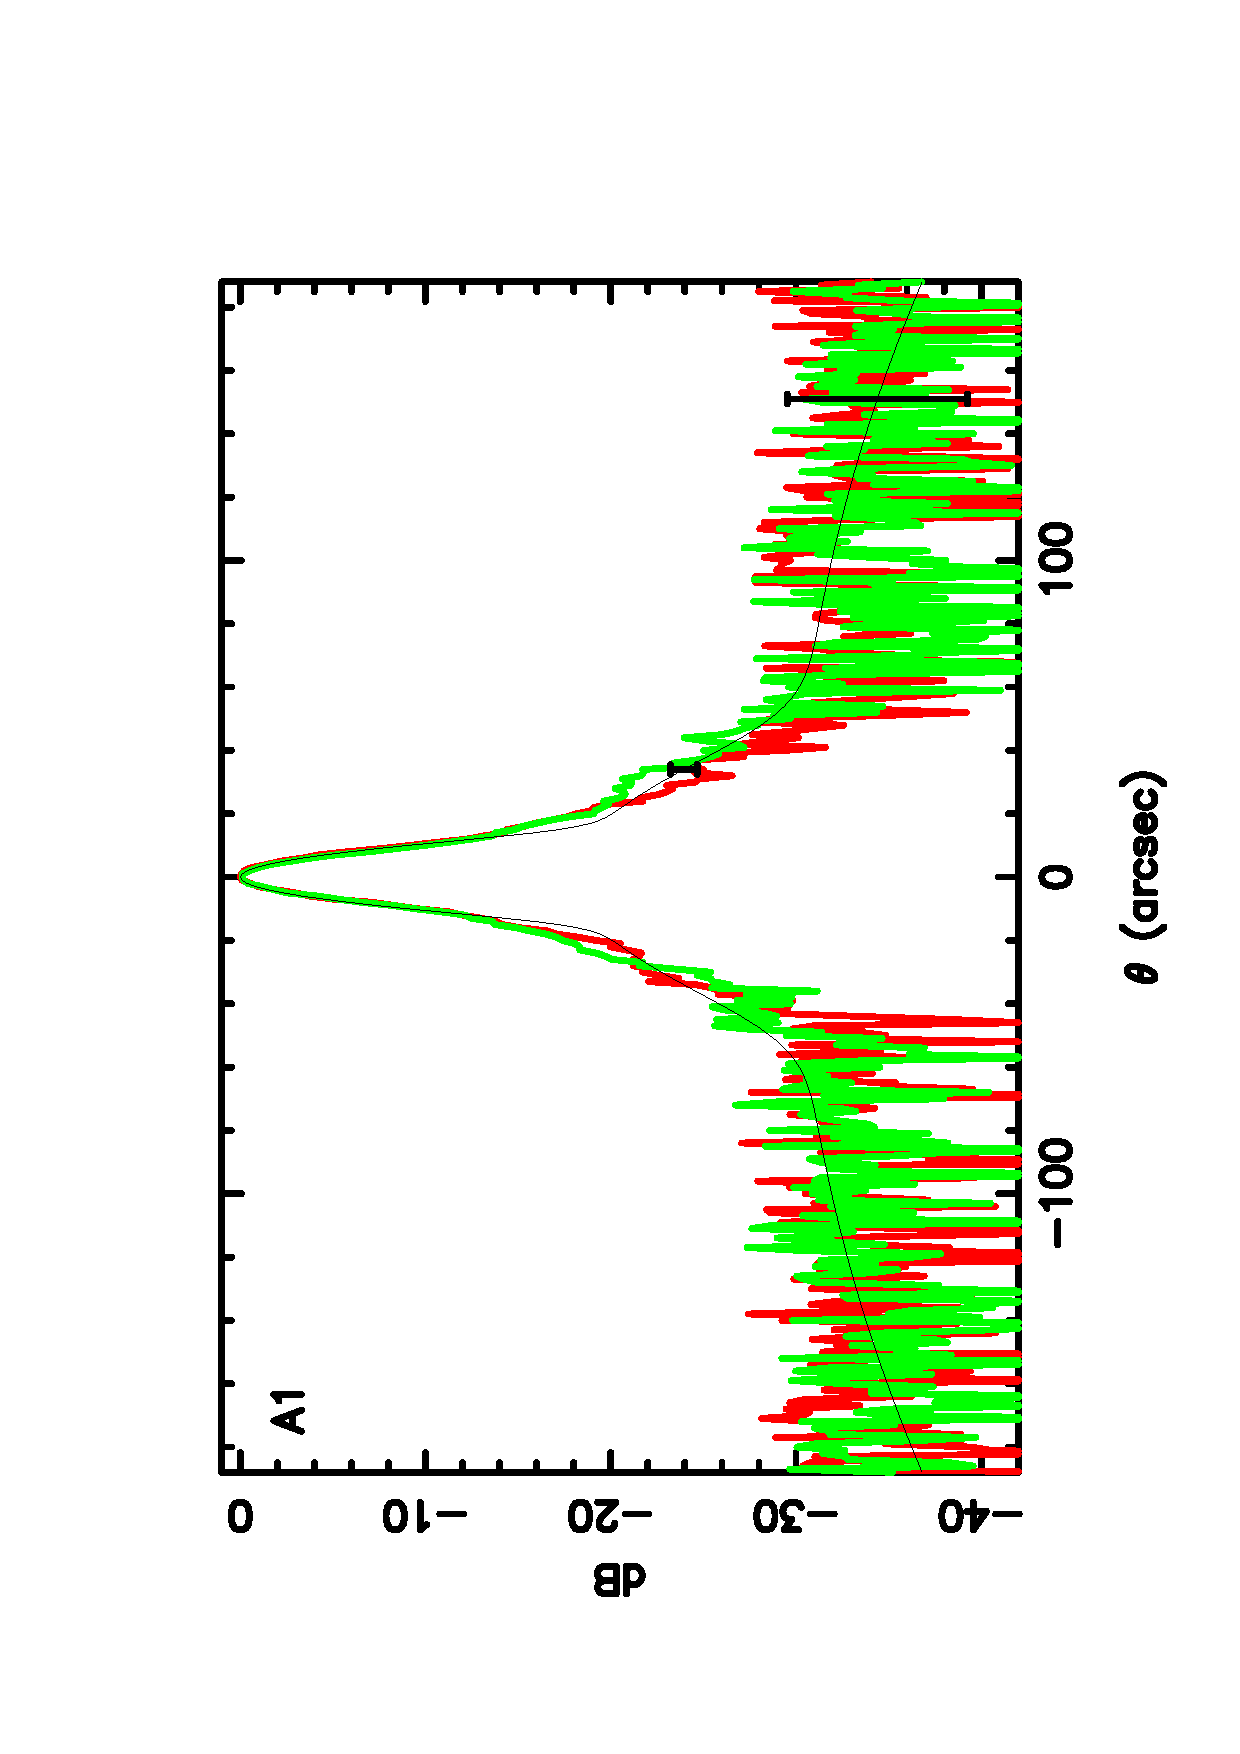
\includegraphics[clip, angle=-90, scale =0.3]{Figures/Array_A1_dB.pdf}
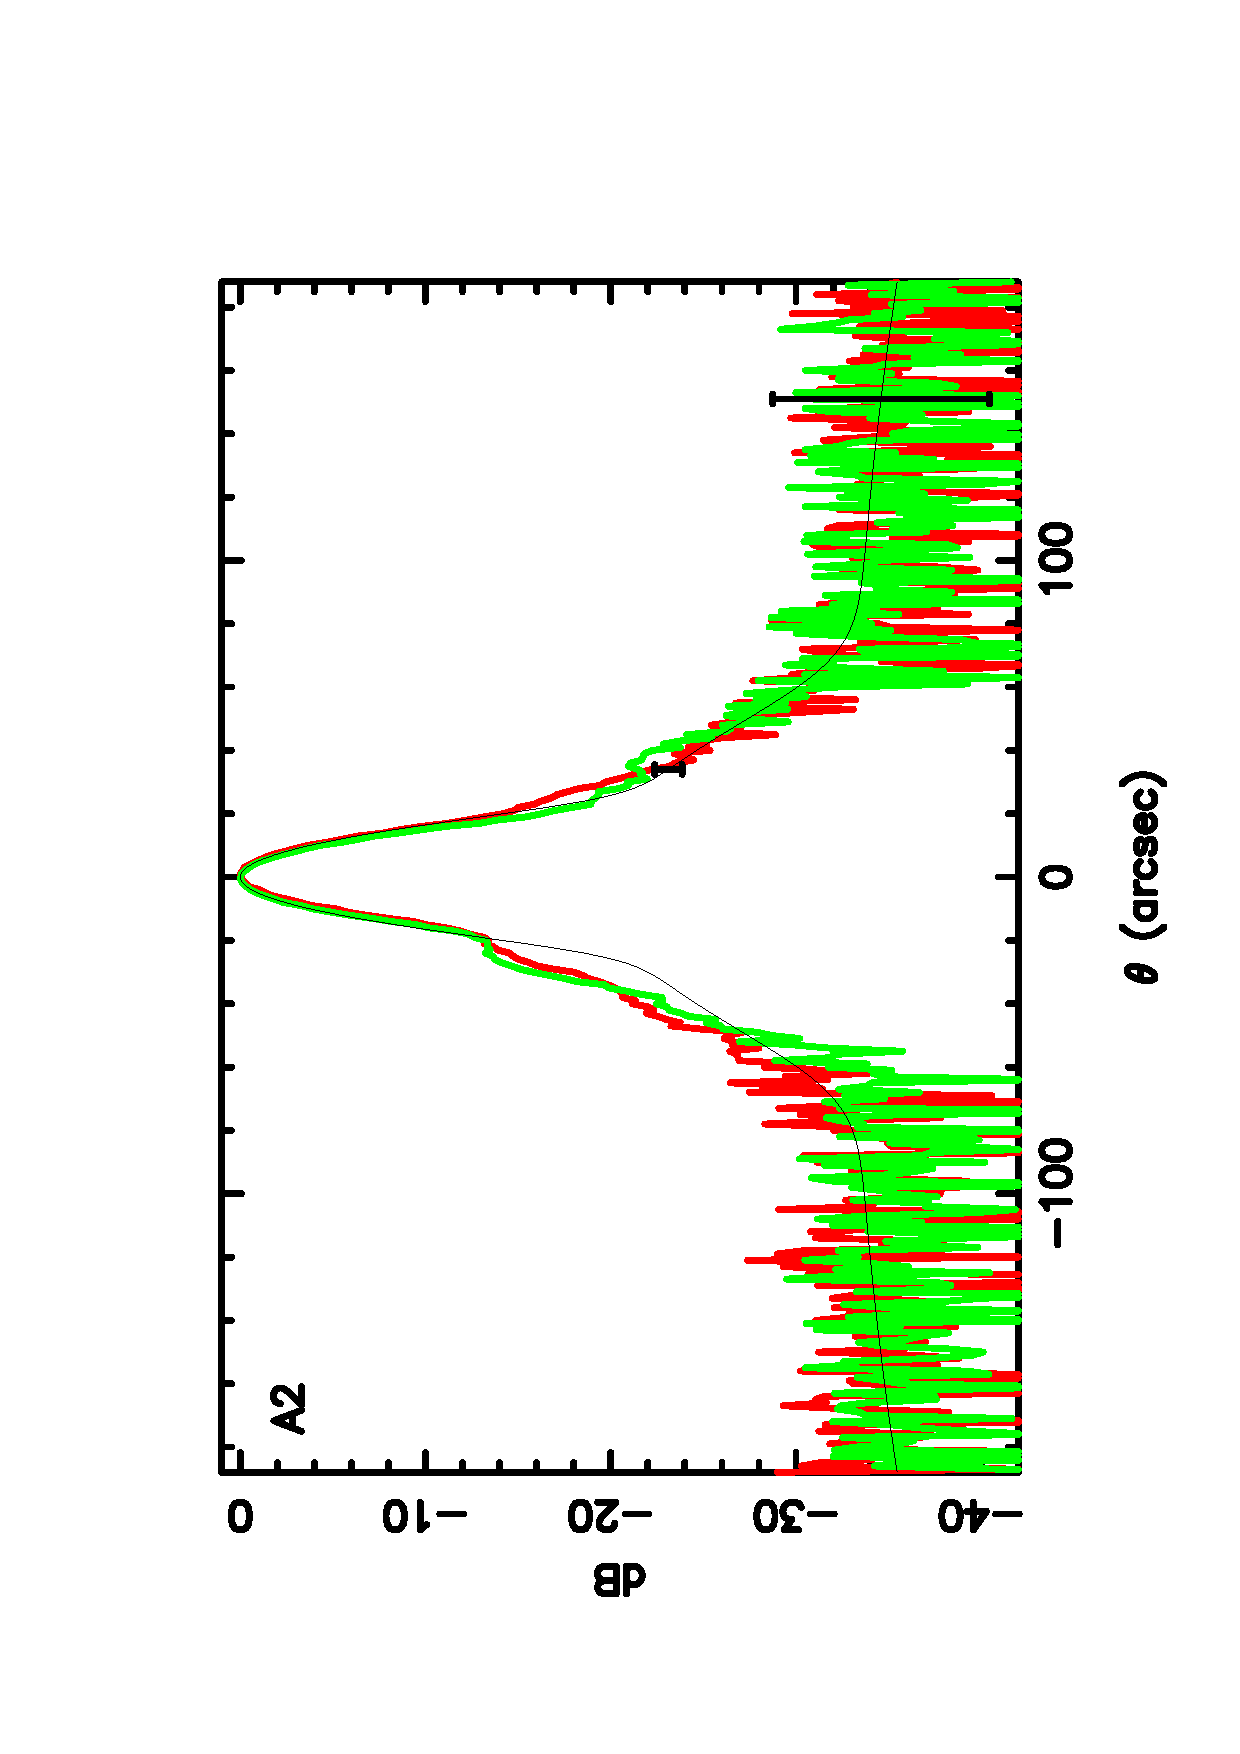
\includegraphics[clip, angle=-90, scale = 0.3]{Figures/Array_A2_dB.pdf}
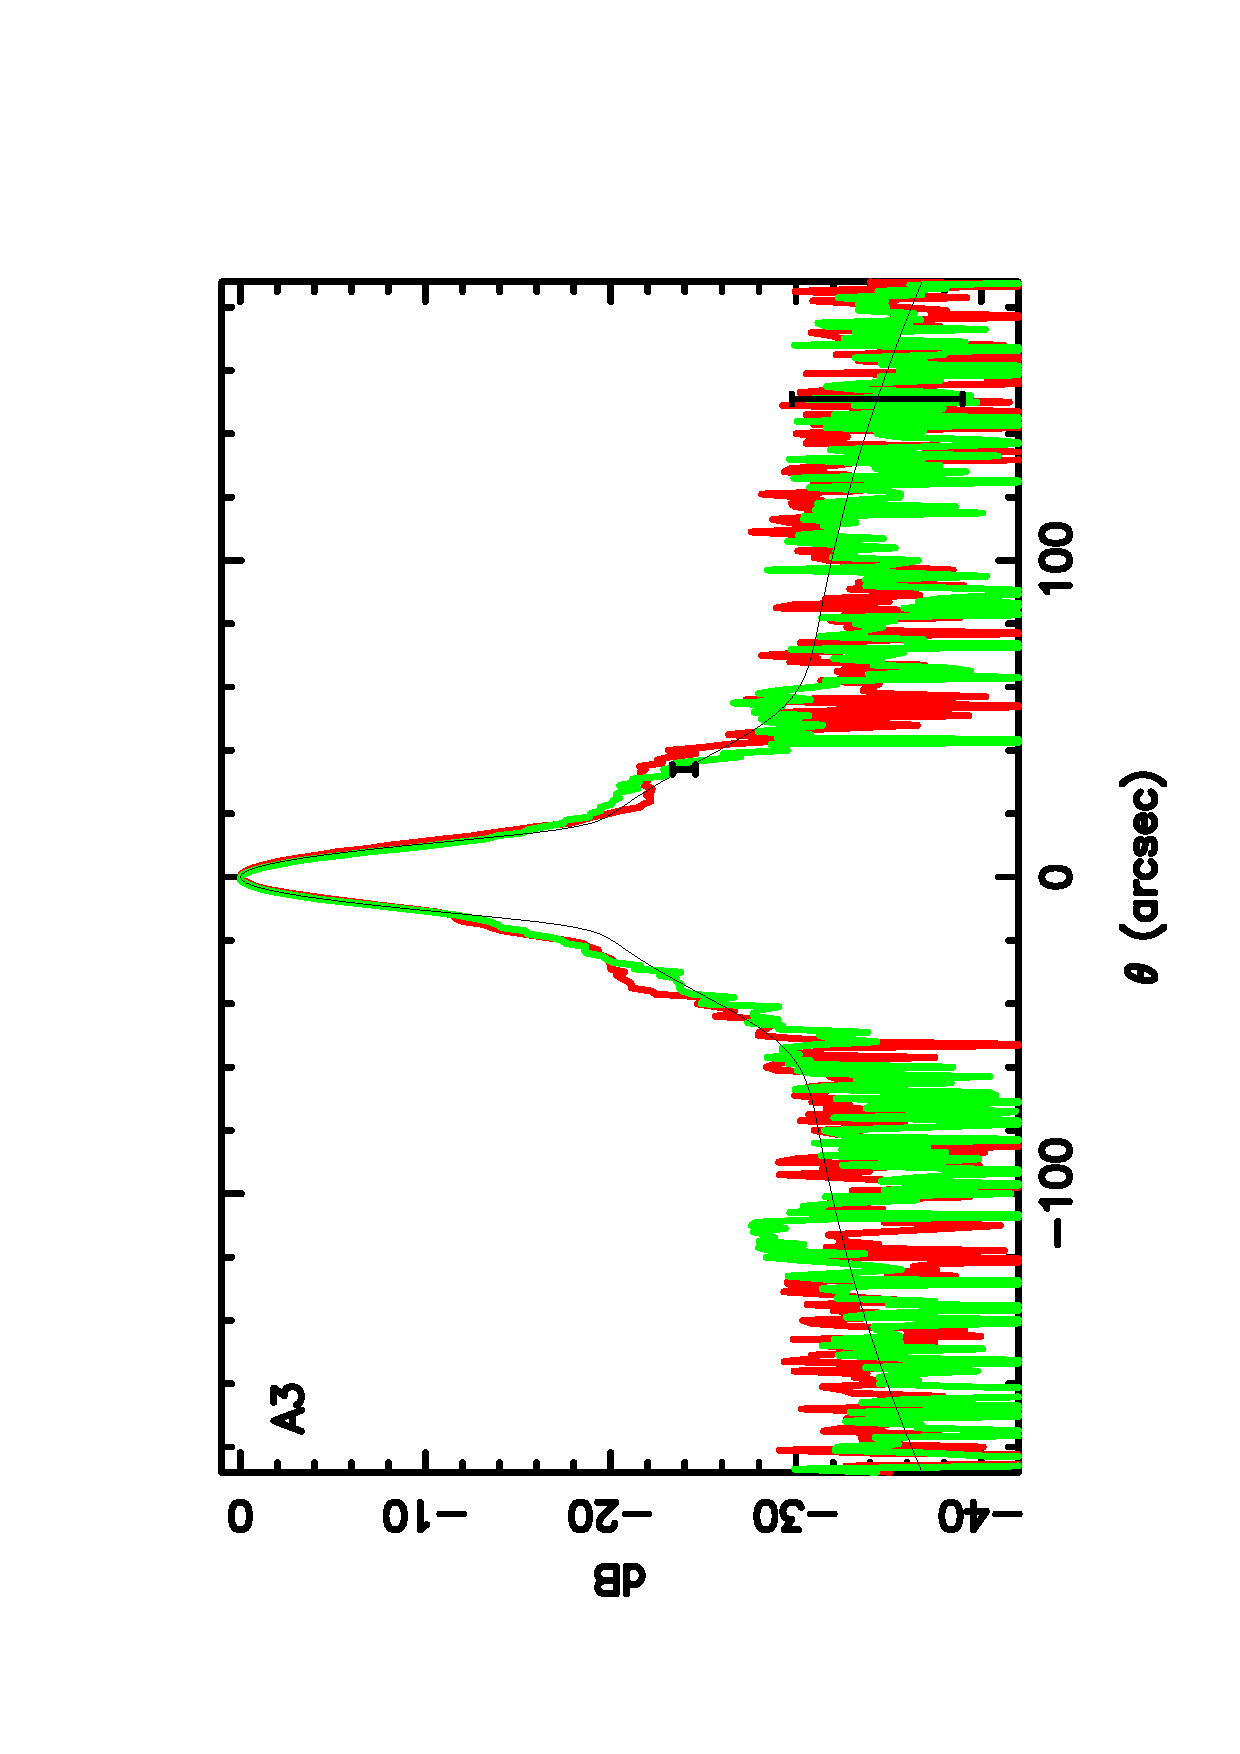
\includegraphics[clip, angle=-90, scale = 0.3]{Figures/Array_A3_dB.pdf}
\caption{Two orthogonal cuts through the beam are shown in red and green and a best fit model made
of three Gaussians is superimposed in black. These cuts were obtained from the high quality map of Uranus on 2017 January 25th.
The main beam starts to depart from the first Gaussian at -12dB. }
\label{fig:beam_dB3}
\end{center}
\end{figure}

The Iram 30-m beam as seen with NIKA2 is shown in
Fig. \ref{fig:beam_db} by means of two orthogonal cuts through Uranus
from a high quality map obtained on 2017 January 25th in excellent conditions
(low opacity $\tau_{225}=0.08$ and elevation $46^{\circ}$).
A model made of three Gaussians centered on the source peak was best
fit {\it by hand} to these cuts and the parameters are reported in
Table \ref{tab:3gauss} [PEUT-ETRE AVANTAGEUSEMENT REPLACED PAR VALEURS DE FLORIAN].
The main beam starts to depart from the first
Gaussian at the level of about -12dB for the three arrays.
We note that for the instrument EMIR on the radiotelescope,
this departure is about -20dB (Kramer, Penalver and Greve 2013).
From parameters in Table \ref{tab:3gauss}, one can estimate that
the source incident power is split about equally between the main beam
and the error beam at 1mm, and these fractions are 70\% and 30\% at 2mm, respectively.
This modelling uses the central
region   $180'' \times 180''$ in size with a uniform noise rms from
a larger area of 8' x 5' on the sky scanned with the arrays. It is expected
that the error beam extend beyond these limits.


\begin{table}
\centering 
\caption[]{Model parameters of the three Gaussian beam.}
\begin{tabular}{|l|l|l|l|l|l|l|}
\hline
               & \multicolumn{3}{c|}{A1 and A3} & \multicolumn{3}{c|}{A2}  \\
\hline
fwhm      & $11.25''$ & $45''$  & $250''$ & $17.75''$ & $56''$  & $420''$ \\
amplitude & 0.984     & 0.015   & 0.0005   &  0.9875   & 0.011   &  0.0005\\
\hline
\end{tabular}
\label{tab:3gauss}
\end{table}


\subsubsection{Beam profile}

[FLORIAN]


%% [Main beam]
\subsection{Main beam}

For NIKA2 main beam characterization, we use \emph{Run9} OTF scans of bright point sources, including primary and secondary calibrators. Namely, we consider scans of Uranus, Neptune, 3C273, 3C84, 0316+413, Vesta and MWC349, whereas we avoid CRL2688 and NGC7027, which are slighltly extended. We perform a conservative data selection from the observing conditions by demanding average elevations $\rm{el} \ge 20°$, zenith opacities as estimated by NIKA2 in the 1mm band $\tau_{1\rm{mm}} \le 0.4$, reasonable lateral focus settings $x, y \le 0.5$mm. After selection cuts, our data set includes 130 OTF scans, which consists of a representative sub-sample of a typical NIKA2 observation campaign.    

  
We consider different methods for the main beam characterization: i) Gaussian fits of the beam profile to benefit from the signal-over-noise increase after azimuthally averaging the signal, ii) Elliptical Gaussian fits of the beam map for a better 2D modeling. Cross-checking the outputs from these complementary methods is an important robustess test of our results.   



\subsubsection{profile-based analysis}

[JEAN-FRANCOIS]

\subsubsection{map-based analysis}

NIKA2 main beam two-dimensionnal distribution is modeled using an elliptical Gaussian. We characterize NIKA2 resolution by giving the \emph{FWHM}, defined as
\begin{equation}
  FWHM = 2 \sqrt{2\ln {2}} \sqrt{\sigma_x\sigma_y},
\end{equation}
where $\sigma_x$ and $\sigma_y$ are the Gaussian standard deviation along minor- and major-axis. To avoid the side lobes contamination, we use masked versions of the beam map, in which an annulus of inner radius $r_{\rm{in}}$ and outter radius $r_{\rm{out}}$ is cut out. Whereas $r_{\rm{out}}$ is conservately set to be $100 arcsec$, $r_{\rm{in}}$ can vary to provide the best 2D Gaussian fit. We checked a posteriori that $r_{\rm{in}}$ distributes as $7 \pm 1.5$ arcsec at 1mm and $13 \pm 4$ arcsec at 2mm, in agreement with settings defined in the profile-based analysis.   

Figure~\ref{fig:fwhm_map} shows FWHM distributions obtained from the elliptical Gaussian fit method.


\begin{figure}
\begin{center}
  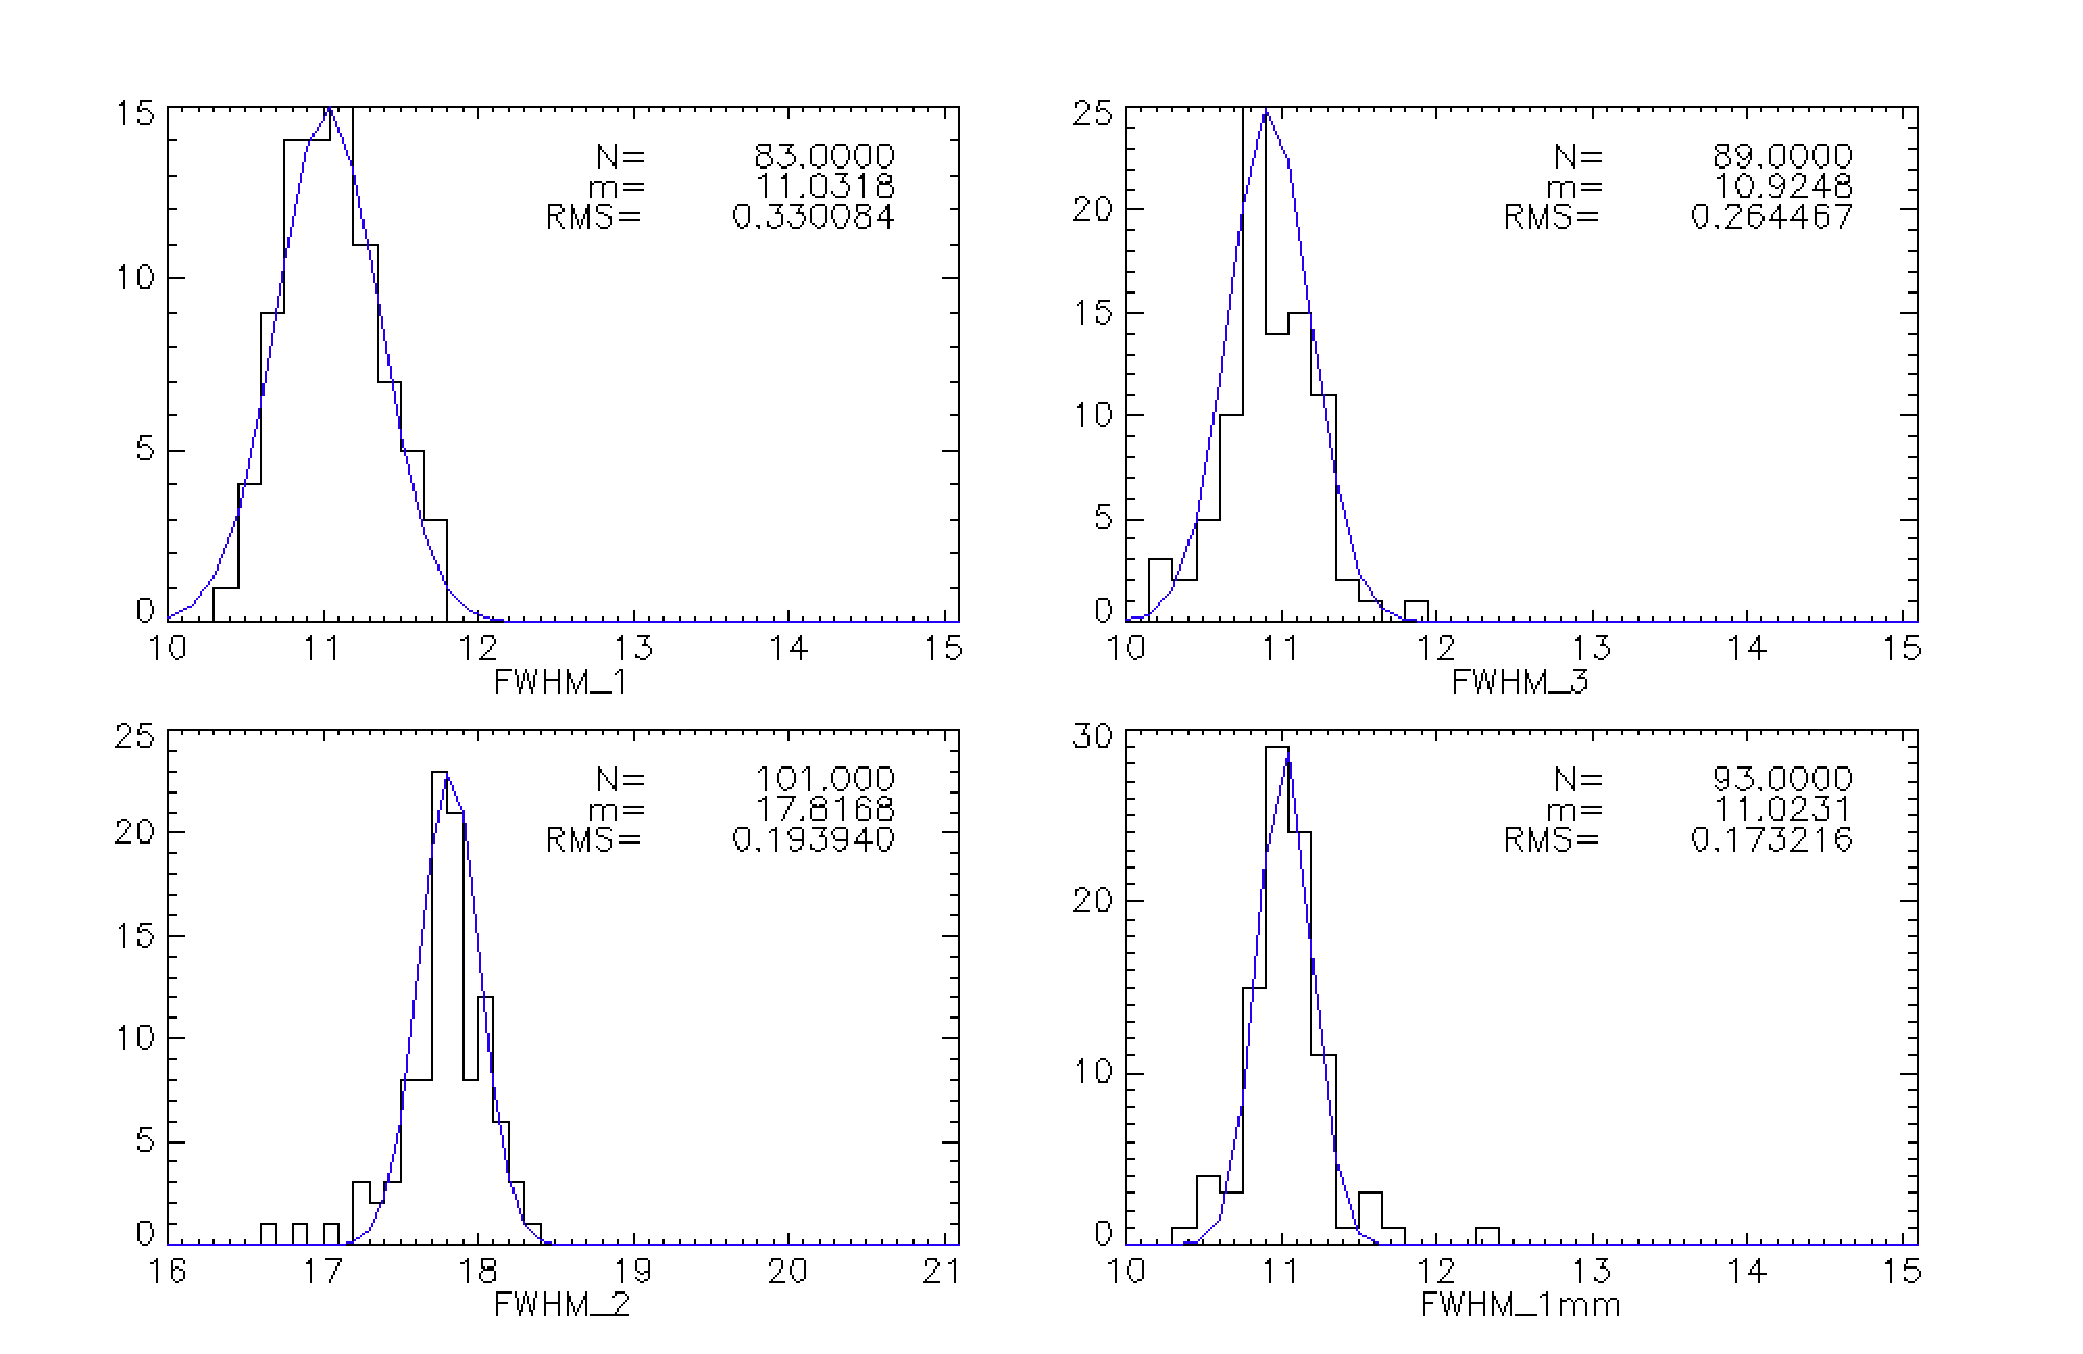
\includegraphics[clip, angle=0, scale=0.4]{Figures/plot_histo_fwhm_run9_calibII_all_nocut.pdf}
\caption{Distribution of the FWHM estimates using 2D Gaussian fits on \emph{N2R9} OTF scans of brigth point sources}
\label{fig:features}
\end{center}
\end{figure}


[A FAIRE:

  AJOUTER UN TABLEAU DE RESULTATS


  AJOUTER LES PLOTS DE STABILITE EN FONCTION DE ELEVATION, TAU

]



